%%
%% This is file `example_DarkConsole.tex',
%% generated with the docstrip utility.
%%
%% The original source files were:
%%
%% examples_kmbeamer.dtx  (with options: `DarkConsole')
%% Copyright (c) 2011-2017 Kazuki Maeda <kmaeda@kmaeda.net>
%% 
%% Distributable under the MIT License:
%% http://www.opensource.org/licenses/mit-license.php
%% 

\documentclass{beamer}

\usepackage{lipsum}             % for dummy text
\usepackage{stix}               % use the STIX font (of course you can delete this line)
\usepackage{nicefrac}

\usetheme{DarkConsole}

\title{Função \(\lambda \)-Modular}
\subtitle{MM413 - Variável Complexa}
\author{Nestor Aponte\footnote{\texttt{n267452@dac.unicamp.br}}}

\begin{document}

\begin{frame}
  \maketitle
\end{frame}

%\begin{frame}{Outline}
%  \tableofcontents
%\end{frame}

\section{Retículos}

\newcommand{\C}{\mathbb{C}}
\newcommand{\R}{\mathbb{R}}
\newcommand{\Z}{\mathbb{Z}}
\newcommand{\Ha}{\mathbb{H}}

\begin{frame}{Definição (\emph{Retículo})}
  \vspace{-0.2cm}
    \[\Z w_1 + \Z w_2 = : \Lambda \subset \C \ \ \Big| \ \ w_j \in \C \text{ \ e \ }\frac{w_2}{w_1} =: \tau \notin \R\]
  \begin{figure}
    \centering
    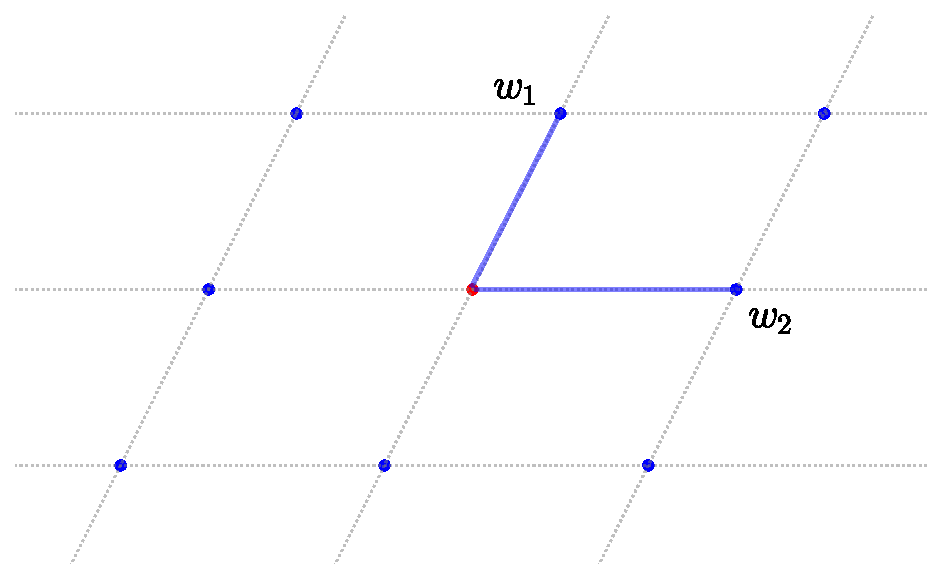
\includegraphics[width = 0.8\linewidth]{ret.pdf}
  \end{figure}
   
%  \textcolor{midyellow}{Proposition.} Sendo \((w_1, w_2)\) uma \emph{base} do \(\Lambda\) as mudanças de base estão dadas por transformações \(T \in \operatorname{SL}_2(\Z)\).

\end{frame}

\begin{frame}{Propriedades}

  \parbox[a]{0.7\textwidth}{
  \textcolor{midyellow}{\(\square\) 1.1.} As mudanças de base em \(\Lambda \) estão dadas por tranformações \(T \in \operatorname{SL}_2(\Z)\). 
  \[\underbrace{\begin{bmatrix}
    a & b \\ c & d 
  \end{bmatrix}}_{T} \overbrace{\begin{bmatrix}
    w_2 & \textcolor{gray}{\overline{w_2}}\\ w_1 & \textcolor{gray}{\overline{w_1} }\\ 
  \end{bmatrix}}^{\text{invertível}} = \begin{bmatrix}
    w_2' & \textcolor{gray}{\overline{w_2'}}\\ w_1'& \textcolor{gray}{\overline{w_1'}}
  \end{bmatrix}\] %\ \Big| \  \begin{bmatrix}
  %  a & b \\ c & d 
  %\end{bmatrix} =: T \in \operatorname{SL}_2(\Z)\]
\pause
  \textcolor{midyellow}{\(\blacksquare\) 1. (\emph{Base Canônica})} Para cada \(\Lambda\) \(\exists (w_1, w_2) : \operatorname{Im}\tau > 0, \ |\operatorname{Re}\tau| \leq \nicefrac{1}{2}\) e \(|\tau| \geq 1\).  
  }
  \pause 
  \parbox[b]{0.25\textwidth}{
  \begin{figure}
    \centering
    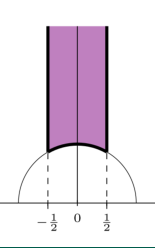
\includegraphics[width = 0.85\linewidth]{mf4FundRegionTau.pdf}
  \end{figure}
   \vspace{-2.3cm}
  }
\end{frame}

\section{\(\wp\)-função de Weierstrass}
\begin{frame}{\emph{\(\wp\)-função de Weierstrass}}
  \[\wp(z):= \frac{1}{z^2} + \sum_{w \in \Lambda^*} \frac{1}{(z-w)^2} + \frac{1}{w^2}\]
  \- \vspace{0.3cm} \\ 
  \textcolor{midyellow}{\(\square\) 1.2.} \textcolor{midyellow}{i.} \(\wp(z)\) converge uniformemente em compactos e é uma função \emph{elíptica}\footnote{\(\wp(z+w) = \wp(z), \ \forall w \in \Lambda\)} par de períodos \(w_1\) e \(w_2\).  \pause \\
  \vspace{0.3cm}
  \textcolor{midyellow}{ii.} Sendo \(G_k :=\sum_{w \in \Lambda^*} w^{-2k}\) (\emph{Eisenstein Series}), a \(\wp\)-função de Weierstrass safisfaz a equação: 
  \begin{align*}
    \wp'(z)^2 &= 4\wp(z)^3 - 60G_2\wp(z) - 140G_3  \\
    &= 4 (\wp(z) -e_1)(\wp(z) -e_2)(\wp(z) -e_3),
  \end{align*} 
  onde \(e_1 = \wp(\nicefrac{w_1}{2})\), \( e_2 = \wp(\nicefrac{w_2}{2})\) e \(e_3 = \wp(\nicefrac{w_1+w_2}{2})\).
\end{frame}

\section{Função \(\lambda\)-Modular}
\begin{frame}{Função \(\lambda\)-Modular}
  \[\frac{e_3-e_2}{e_1-e_2} =: \lambda(\tau) =  \left(\frac{a + b\tau}{c + d\tau}\right)  \ \Big| \ \begin{bmatrix}
    a & b \\ c & d
  \end{bmatrix} \equiv \begin{bmatrix}
    1 & 0 \\ 0 & 1
  \end{bmatrix} \ (\operatorname{mod} \ 2) \]%\ \textcolor{gray}{\leq \operatorname{SL_2(\Z)}}\] 
  \pause
  \- \vspace{0.1cm} \\ 
  \textcolor{midyellow}{\(\blacksquare\) 2.} \(\lambda : \Omega \cup \Omega' \simeq \C\setminus \{0,1\}\) (conforme) e verifica \(\tau:  0, 1, \infty \mapsto  1, \infty, 0\) respetivamente.   
  \vspace{0.1cm}
  \begin{figure}
    \centering
    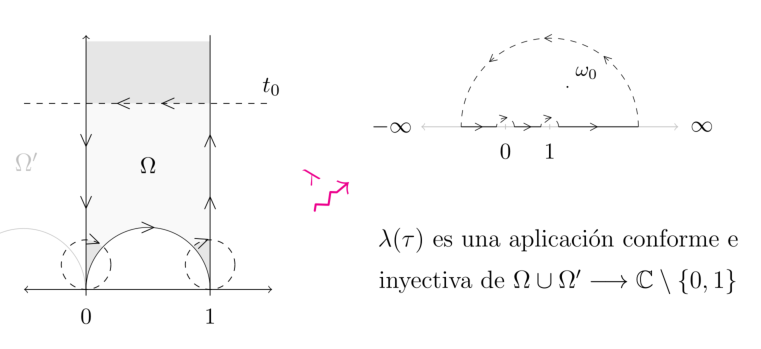
\includegraphics[width = 0.75\linewidth]{Teo1.pdf}
  \end{figure}
\end{frame}

\begin{frame}
  \textcolor{midyellow}{\(\blacksquare\) 3.} Todo \(\tau \in \mathbb{H}\) é equivalente a menos de congruência \((\operatorname{mod} \ 2)\) a exatamente um ponto \(S_\tau \in \overline{\Omega} \cup \Omega'\).
  \vspace{0.1cm}
  \begin{figure}
    \centering
    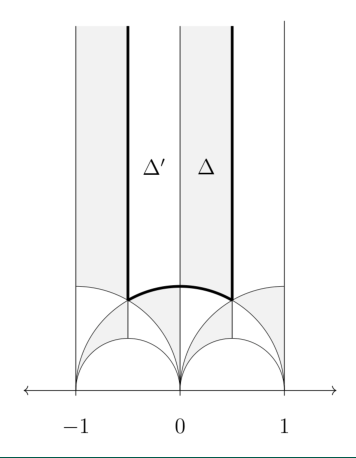
\includegraphics[width = 0.4\linewidth]{Teo2.pdf}
  \end{figure}
\end{frame}

\section{Picard}
\begin{frame}{Teorema (pequeno) de Picard - A ideia}
  \hrule 
  \vspace{0.5cm}
  \textcolor{midyellow}{\(\blacksquare\) (\emph{Picard})} Uma função inteira cuja imagem omite dois ou mais valores complexos diferentes é constante. 
  \[f \in \mathcal{O}(\C) : \operatorname{Im} f \subset \C \setminus \{a,b\} \ \Rightarrow \ f \text{ constante}\]
  \hrule 
  \vspace{0.5cm} \pause 
  \begin{itemize}%[label = \(\rightarrow\)]
    \item \(\displaystyle \widetilde{f}(z) = \frac{f(z) -a}{b-a} \text{ constante } \Rightarrow \  f(z) \text{ constante}\), podemos supor então de inicio \(a = 0, \ b=1\). 
  \end{itemize}
\end{frame}
\begin{frame}
  \begin{itemize}
    \item Pelo \(\blacksquare\) 2. \hspace{-0.5cm} \(\exists \tau_0 \in \Ha : \lambda(\tau_0) =  f(0)\) e \(\lambda'(\tau_0) \neq 0\). Pelo \(\blacksquare\) (\emph{TFI}) \(\exists \lambda_0^{-1}: \Delta_0 \to D\) e por contínuidade \(\exists \Omega_0 : f(\Omega_0) \subset \Delta_0\).  
    \vspace{0.2cm}
  \begin{figure}
    \centering 
    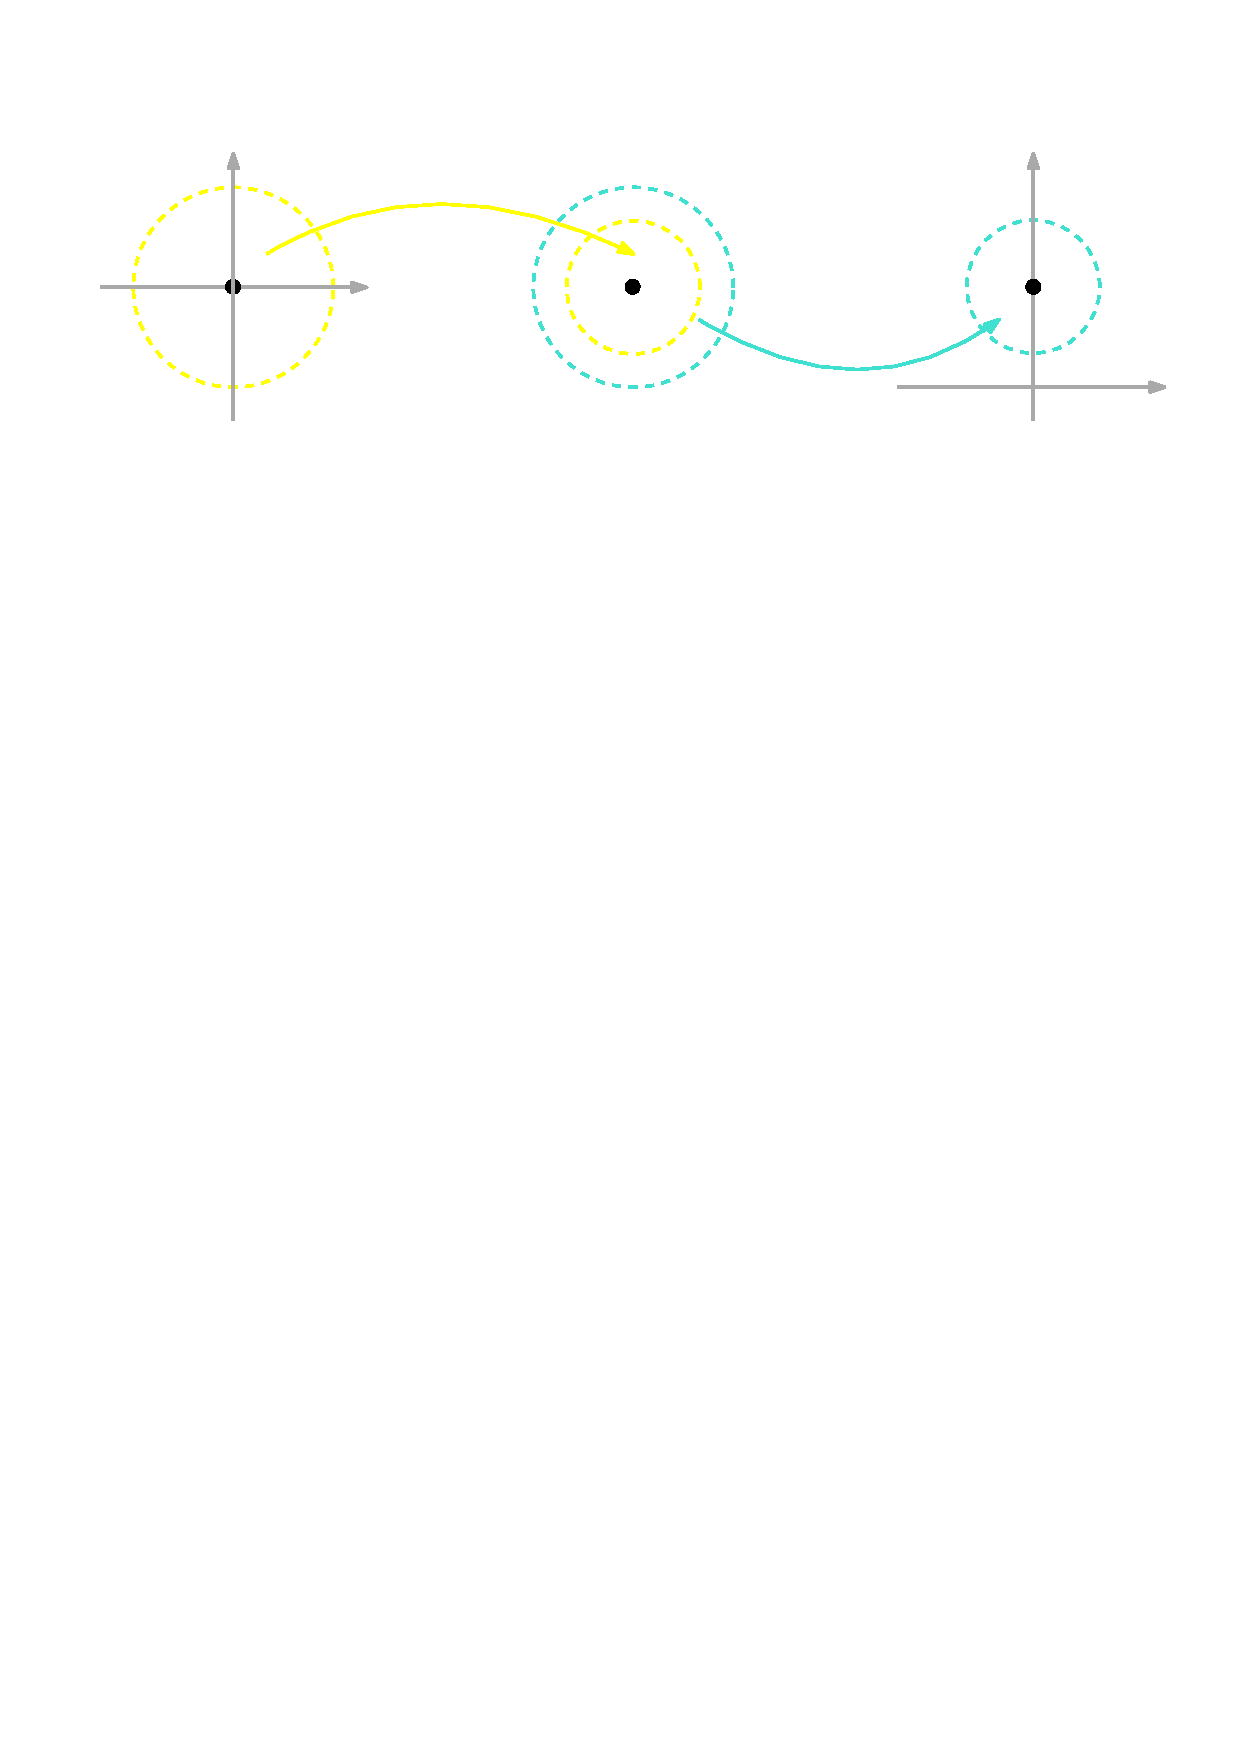
\includegraphics[width = 0.8\linewidth]{graph1.pdf}
  \end{figure}
  \vspace{0.2cm}
  Considere a função \(\displaystyle h: \Omega_0 \to D\) tal que \(h(z)= \lambda_0^{-1}(f(z))\). Note que \(f(z) = \lambda_0(h(z))\) em \(\Omega_0\) e \(\operatorname{Im} h > 0\). 
\end{itemize}
\end{frame}
\begin{frame}
  \begin{itemize}
  \item Após usando o \(\blacksquare\) 3. + Contínuação Analítica (em termos de curvas) pode-se mostrar que  \(h\) é de fato inteira.  \pause
  \vspace{0.5cm}
  \item \(\displaystyle |e^{h(z)}|  = |e^{ix}e^{-y}|\leq 1\) pois \(y>0\). Pelo \(\blacksquare\) (\emph{Liouville}) \(h(z) = \lambda^{-1}_0(f(z))\) é constante assim como \(f(z) = \lambda_0(h(z))\).
  \end{itemize}
\end{frame}

\section{De graça}

\begin{frame}{Gráficos}
  \begin{figure}
      \centering
      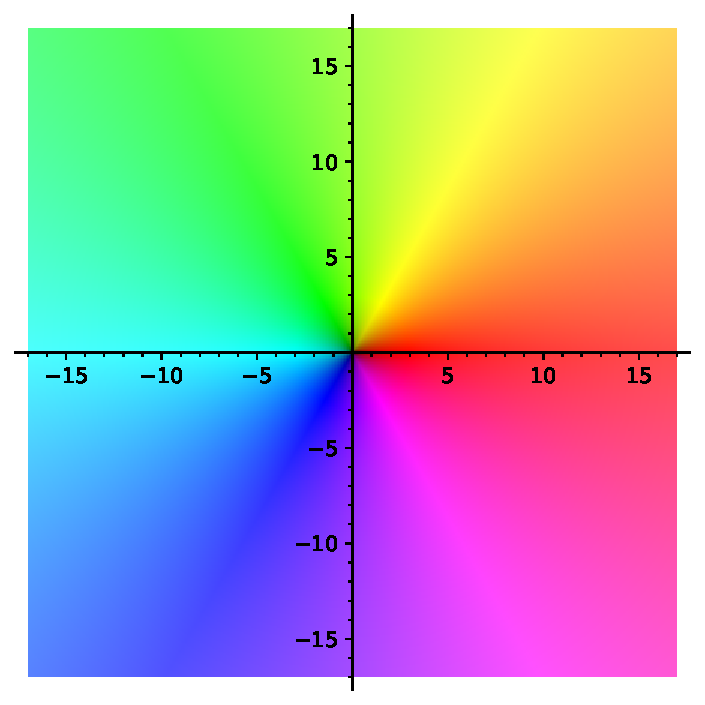
\includegraphics[width = 0.5\linewidth]{z.pdf} 
      \[f(z) = z\]
  \end{figure}
\end{frame}

\begin{frame}{Teorema (grande) de Picard - nem ideia}
  \textcolor{midyellow}{\(\blacksquare\) (\emph{Picard})} Sejam \(f \) holomorfa numa vizinhança furada de \(z_0\) singularidade esencial da \(f\). Então, \(\operatorname{Im}f \subset \C\setminus\{a\}\) e cada valor é tomado infinitas vezes.
  \vspace{0.3cm}
  \[\text{\textcolor{midyellow}{Exemplo.\hspace{0.1cm}}}f(z) = \sin\left(\frac{1}{z}\right) \text{ perto do } 0\]
  \begin{columns}
\column{0.3\textwidth}
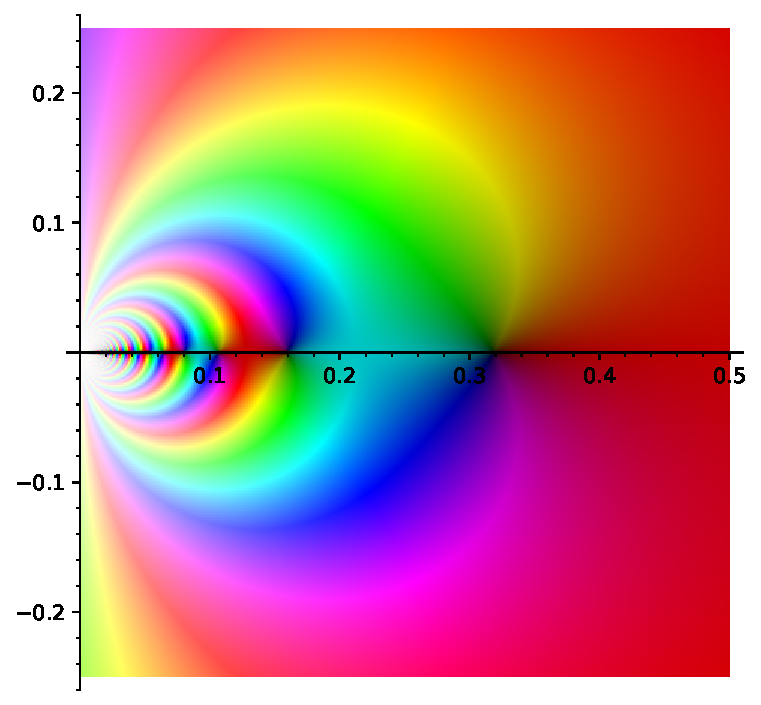
\includegraphics[width=\linewidth]{1.pdf}
\centering \(\epsilon = \nicefrac{1}{4}\)

\column{0.3\textwidth}
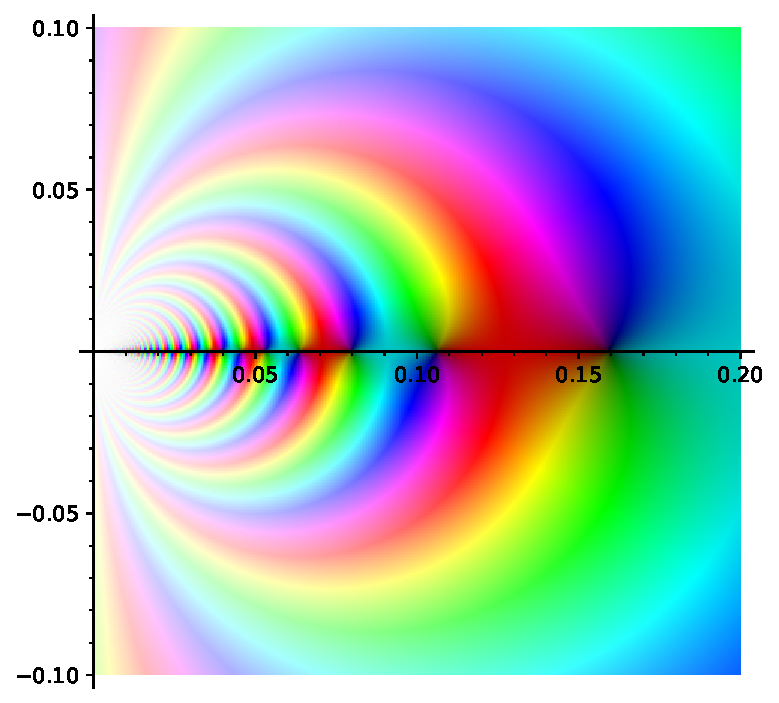
\includegraphics[width=\linewidth]{2.pdf}
\centering \(\epsilon = \nicefrac{1}{10}\)

\column{0.3\textwidth}
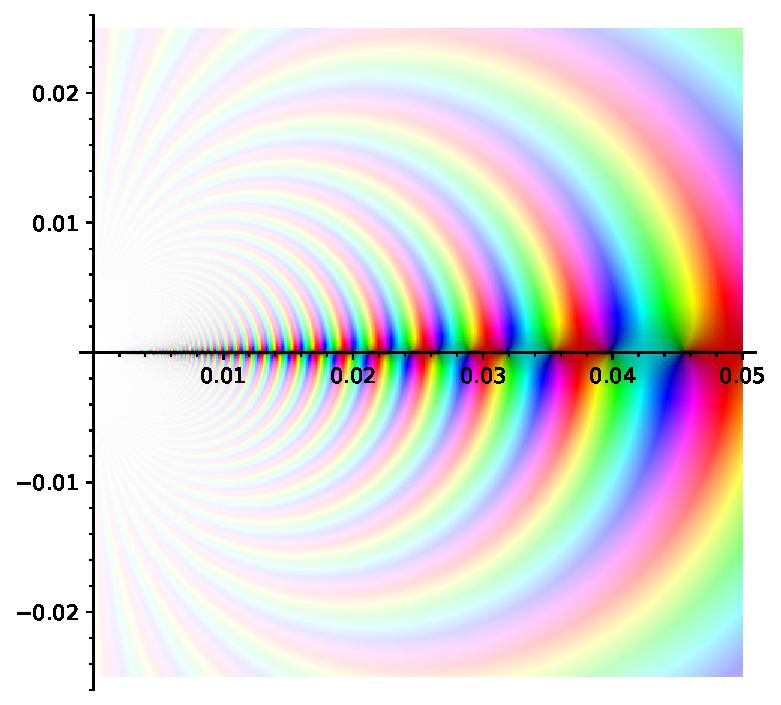
\includegraphics[width=\linewidth]{3.pdf}
\centering \(\epsilon = \nicefrac{3}{100}\)

\end{columns}
\end{frame}

\end{document}
